\chapter{Grundlagen}
\label{Grundlagen}
Das Ziel dieser Arbeit besteht darin aus einem UML-Modell ein GWT-Projekt zu
generieren. Zur Verständnis werden in diesem Kapitel einige wichtige
Grundlagen erläutert.
% ---------------------------------------------
% MDA
% ---------------------------------------------
\section{Model Driven Architecture} \label{MDA}
Model Driven Architecture (dt. Modellgetriebene Architektur), kurz MDA, stellt
einen Ansatz zur Softwareentwicklung dar. Dieses Konzept ist 2001 von der
Object Management Group (OMG) veröffentlicht worden und gilt heute als
Standard. Hierbei werden Richtlinien zur Spezifikation in Form von Modellen vorgegeben.
Aus diesen Modellen, die formal eindeutig sind, wird dann mithilfe von Generatoren
automatisch der benötigte Code erzeugt. Ziel der MDA-Architektur ist es, den gesamten Prozess der Softwareerstellung in möglichst plattformunabhängigen Modellen darzustellen, sodass die Software zu einem hohen Anteil automatisch durch Transformationen von Modellen erzeugt werden kann. Die dabei entstehenden Transformatoren können eine hohe Wiederverwendbarkeit und Wartbarkeit sicherstellen.\cite[S. 79 f.]{bib:MDA1}\\
Bei den Modellen handelt es sich im Speziellen, um das Platform Independent Model und das Platform Specific Model, welche bei diesem Projekt auf das Metamodell der UML 2.4 Anwendung fanden.
Was dies genau bedeutet und wie die verschiedenen Modelle zu verstehen sind, wird in dem folgenden Abschnitt erläutert

\subsection{Platform Independent Model und Plattform Specific Model} \label{PIMPSM}
Das Platform Independent Model (PIM, dt. plattformunabhängiges Modell) stellt ein
Softwaresystem dar, das unabhängig von der technologischen Plattform ist. Zudem wird die konkrete technische Umsetzung des Systems nicht berücksichtigt. In dem PIM
sind alle Anforderungen erfasst. Alles, was es im System zu spezifizieren gibt, ist definiert,
jedoch komplett frei von der später folgenden Implementierung. Somit ist nicht nur eine
einzige Implementierung des Systems möglich, sondern durchaus mehrere
unterschiedliche.
Werden nun die Funktionalitäten kombiniert, die im Platform Independent Model definiert sind, mit den Designanforderungen der gewünschten Plattform, so entsteht das Platform Specific Model (PSM, dt. plattformspezifisches Model). Dies geschieht über Modelltransformationen. Das nun entstandene PSM kann durch weitere Transformationen immer spezifischere Modelle erstellen, bis letztendlich der Quellcode für eine Plattform generiert wird. Im Gegensatz zum PIM, welches nur die
fachlichen Anforderungen definiert, werden beim PSM auch die technischen Aspekte
eingebunden.\cite[S.377 ff.]{bib:MDA2}\cite{bib:MDA3}\\ 
 
Allerdings ist zu beachten, dass es sich bei PIM und PSM um relative Konzepte handelt. 
In diesem Projekt sind sowohl M1 als auch M2 Modell im Bezug auf GWT als PIM zu betrachten. Die eigentliche Spezifizierung für GWT erfolgt erst bei der Model-To-Text Transformation im Generator.
% ---------------------------------------------
% GWT
% ---------------------------------------------
\section{GWT}
\label{GWT}
Das Google Web Toolkit, kurz GWT, ist ein open-source Projekt von Google. Es
dient der Entwicklung von Webanwendungen mittels Java. Dabei übersetzt der GWT
Compiler den gesamten Java Source-Code in JavaScript Code.
Zudem werden während der Übersetzung Code Optimierungen vorgenommen, welche u.A.
das Löschen von nicht benötigtem Code, z.B beim Einsatz von mehreren
Browsern als Plattformen, betreffen. 

Weiterhin bietet GWT die Möglichkeit zur Interaktion mit JavaScript durch
das JavaScript Native Interface, kurz JSNI.
Dadurch können JavaScript Bibliotheken angebunden bzw. verwendet oder die
Nutzung von JSON erleichtert werden \cite[S. 4-9]{bib:GWTinAction}\cite[S.
237-238]{bib:GWToReilly}.

Darüber hinaus ist dadurch eine Kommunikation mit dem Backend
möglich. Zusätzlich kann diese Kommunikation durch Remote Procedure Calls,
kurz RCPs, u.A. mittels RequestBuilder oder GWT-RCP erfolgen. Beide setzen auf
dem XMLHttpRequest JavaScript Objekt auf, welches die Kommunikation zwischen dem
Browser und dem Server ohne Seitenneuladen erlaubt. Der RequestBuilder ist ein
Wrapper für das genannte JavaScript Objekt und GWT-RCP ermöglicht den Austausch
von konkreten Java Objekten \cite[S. 16]{bib:GWTinAction}\cite[S.
222]{bib:GWToReilly}.

Dies zeigt einen kurzen Einblick in die verschieden Möglichkeiten mit
GWT, welche folgend nicht näher erläutert werden, weil eine Generierung einer
GWT Frontend Anwendung ohne Server Kommunikation erfolgen soll.

Der Einsatz mit GWT ist flexibel und durch den GWT Compiler wird 
eine bessere Laufzeitausfürhung der Webanwendung erlangt\cite{bib:GWTStarted}.
Dies sind 2 Vorteile des Nutzens von GWT. Zusätzlich sind die durch Google
gebotenen Architekturkonzepte durch u.A. Model-View-Presenter, kurz MVP, ein
Ansatz und Grund einen Generator für GWT Frontend Anwnedungen zu schreiben.
Dafür werden im weiterem Verlauf MVP, UiBinder sowie GIN erläutert, welche die
Grundlage der umzusetzenden Architektur bilden.

\subsection{MVP}
\label{MVP}
MVP (Model-View-Presenter) ist ein Design Pattern. Es ist ähnlich dem MVC
(Model-View-Controller). Google beschreibt den Nutzen des MVP Patterns in der
Einbindung von Testfällen in einer GWT Anwendung. Darüber hinaus kann dieses
Pattern auch genutzt werden um eine GWT Anwendung für verschiedene Plattformen
verfügbar zu machen z.B. für Browser auf mobilen Endgeräten oder auf dem
Desktop.
\begin{figure}[htbp]
\begin{center}
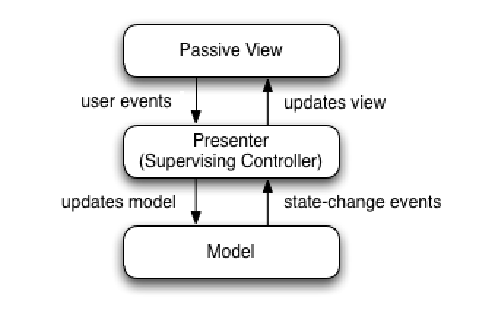
\includegraphics{./img/MVP.pdf}
\caption{Visualisierung des MVP Patterns \cite{bib:MVP1}}\label{Fig:MVP}
\end{center}
\end{figure}\\
Bei MVP übernimmt der Presenter die Logik und die View ist einfach gehalten
\cite{bib:MVP2}. Dies sorgt für eine klare Trennung zwischen Model und View (vgl.
Abbildung \ref{Fig:MVP}). Wohingegen bei MVC die View das Model kennt
\cite{bib:MVCvsMVP}. Der Presenter steuert die View und übermittelt die Daten
des Models zur View.
Dadurch wird der einfache Austausch von Views ermöglicht ohne das weitere
Änderungen vorgenommen werden müssen \cite{bib:MVP1}\cite{bib:MVP2}.

In der zu generierenden Anwendung soll das MVP Pattern ohne ein konkretes Model
implementiert werden, da ausschließlich eine GWT Frontend Anwendung generiert
werden soll. Die MVP Struktur ist dabei so umgesetzt, sodass der Presenter als
Interface in dem View Interface enthalten ist und über eine Activity definiert
wird, welche zusätzlich für das Event handling und die Datenbeschaffung verantwortlich
ist. Die konkrete Implementierung der View beinhaltet das Presenterobjekt, damit
dadurch die Aktionen der View Komponenten (bei GWT Widgets) an den Presenter
übergeben werden können.

\subsection{UI-Binder}
\label{UIBinder}
% ---------------------------------------------
% GIN
% ---------------------------------------------
\section{Dependency Injection mittels GIN} \label{GIN}
Bei Dependency Injection handelt es sich um einen Begriff aus der
objektorientierten Programmierung, welcher zuerst von Martin Fowler 2004
verwendet worden ist \cite{bib:DI}. Beim Dependency Injection handelt es sich um
ein Verfahren, bei dem zur Laufzeit eines Programmes zusätzliche Informationen,
beispielzweise beim Aufruf einer Funktion, zur Verfügung gestellt werden. Dies
wird von einem extra Dependency Injection Framework vorgenommen, in dieser
Arbeit wird handelt es sich dabei um das GIN Framework.

\subsection{GIN}
Das GIN-Framwork, ist ein Framwork für Dependency Injection, es wurde von Google
für GWT entwickelt \cite[GIN]{bib:gin}. GIN setzt auf Google Guice
\cite[Guice]{bib:guice} auf und erweitert die Java Dependency Injection für den
speziellen Anwendungsfall von GWT.  GIN wurde direkt in den GWT Generator
eingebaut, wodurch es möglich ist die Dependency Injection teilweise schon zur
Compile Zeit einzufügen, dies Sorgt dafür das es kaum Laufzeit Overhead gibt.

Guice wurde 2008 von Google für Dependency Injection mit Java entwickelt und war
das erste Framwork, das Dependency Injection mit Hilfe von Annotationen
ermöglicht hat. Bei Guice werden mittels bind-Befehlen eine Verbindung zwischen
Interfasen und deren konkreten Klassen hergestellt, dadurch sind die konkreten
Implementierungen leichter Austauschbar.

